\documentclass[tikz,border=2pt,11pt]{standalone}
\usetikzlibrary{arrows.meta}
\usetikzlibrary{calc}
\usetikzlibrary{positioning}
\usetikzlibrary{fit}
\usepackage{amsmath}
\usepackage{amssymb}
\usepackage{graphicx}
\usepackage{tikz}
\providecommand*{\lemmaautorefname}{Lemma}
\providecommand*{\propositionautorefname}{Proposition}
\providecommand*{\corollaryautorefname}{Corollary}
\providecommand*{\definitionautorefname}{Definition}
\providecommand*{\conventionautorefname}{Convention}
\providecommand*{\exampleautorefname}{Example}
\providecommand*{\remarkautorefname}{Remark}
\DeclareMathOperator{\Con}{Con}
\DeclareMathOperator{\Aut}{Aut}
\DeclareMathOperator{\End}{End}
\DeclareMathOperator{\Sym}{Sym}
\DeclareMathOperator{\Alt}{Alt}
\DeclareMathOperator{\Soc}{Soc}
\DeclareMathOperator{\core}{core}
\DeclareMathOperator{\GL}{GL}
\DeclareMathOperator{\SL}{SL}
\DeclareMathOperator{\PGL}{PGL}
\DeclareMathOperator{\PSL}{PSL}
\DeclareMathOperator{\AG}{AG}
\DeclareMathOperator{\Fr}{Fr}
\DeclareMathOperator{\rank}{rank}
\DeclareMathOperator{\im}{im}
\DeclareMathOperator{\id}{id}
\newcommand{\F}{\mathbb F}
\newcommand{\N}{\mathbb N}
\newcommand{\Z}{\mathbb Z}
\begin{document}
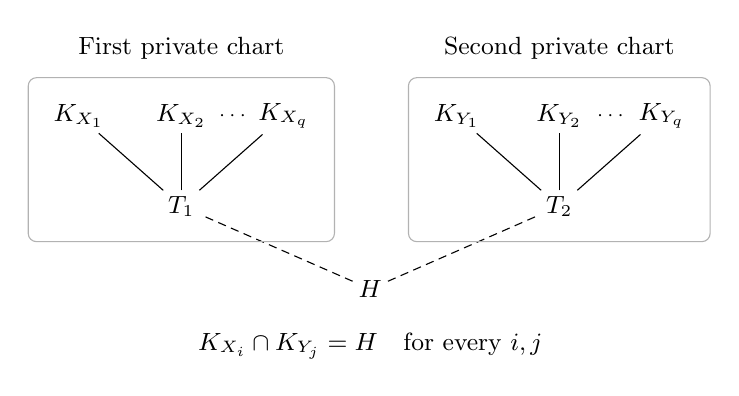
\begin{tikzpicture}[x=1cm,y=1cm,
  witness/.style={font=\small,inner sep=2pt},
  inclusion/.style={densely dashed},
  panel/.style={draw=black!30,rounded corners=3pt,inner sep=7pt}]
\node[witness] (h) at (0,0) {\(H\)};
\node[witness] (t1) at (-2.4,1.05) {\(T_1\)};
\node[witness] (t2) at (2.4,1.05) {\(T_2\)};
\node[witness] (k11) at (-3.7,2.2) {\(K_{X_1}\)};
\node[witness] (k12) at (-2.4,2.2) {\(K_{X_2}\)};
\node[witness] (k1q) at (-1.1,2.2) {\(K_{X_q}\)};
\node[witness] (k21) at (1.1,2.2) {\(K_{Y_1}\)};
\node[witness] (k22) at (2.4,2.2) {\(K_{Y_2}\)};
\node[witness] (k2q) at (3.7,2.2) {\(K_{Y_q}\)};
\node[font=\scriptsize] at (-1.75,2.2) {\(\cdots\)};
\node[font=\scriptsize] at (3.05,2.2) {\(\cdots\)};
\foreach \target in {k11,k12,k1q}{\draw (t1)--(\target);}
\foreach \target in {k21,k22,k2q}{\draw (t2)--(\target);}
\draw[inclusion] (h)--(t1);
\draw[inclusion] (h)--(t2);
\node[panel,fit=(t1)(k11)(k12)(k1q)] (p1) {};
\node[panel,fit=(t2)(k21)(k22)(k2q)] (p2) {};
\node[font=\small,above=3pt of p1] {First private chart};
\node[font=\small,above=3pt of p2] {Second private chart};
\node[font=\small,below=7pt of h] {\(K_{X_i}\cap K_{Y_j}=H\quad\text{for every }i,j\)};
\end{tikzpicture}
\end{document}
